\chapter{Retrossíntese e estratégia em várias etapas}\label{ch:b2:retrosynthesis}

Uma molécula é desenhada no quadro, e ninguém ainda sabe como prepará-la. Testar reações no sentido
direto, a partir do que está na prateleira, não leva a nada: são numerosas demais. O químico trabalha
no outro sentido, do alvo de volta à prateleira, cortando uma ligação de cada vez no papel, cada corte
desfazendo uma reação que se sabe funcionar, até que os pedaços sejam compostos que se podem comprar.
Este capítulo transforma as reações dos capítulos anteriores nesse raciocínio às avessas, e depois
pergunta como julgar a via que ele produz.

\begin{recall}
Do \cref{ch:b2:alkene-redox} ao \cref{ch:b2:wittig}: as reações a desfazer. O volume do 1.º ano: grupos
protetores e acetais, reagentes de Grignard e inversão de polaridade, a síntese de Williamson, a
quimiosseletividade, a oxidação dos álcoois. O volume escolar: a economia atômica.
\end{recall}

\section{Pensar às avessas}

\begin{definition}[Análise retrossintética]\label{def:b2:retrosynthesis:analysis}
A molécula a preparar é a \emph{molécula-alvo}\index{molecula-alvo@molécula-alvo}. A \emph{análise retrossintética}
\index{analise retrossintetica@análise retrossintética} trabalha do alvo de volta a materiais de partida disponíveis,
por etapas cada uma das quais é o inverso de uma reação conhecida; uma etapa retrossintética se escreve
com a seta dupla $\Rightarrow$, lida ``é preparado a partir de''.
\end{definition}

\begin{definition}[Desconexão e síntons]\label{def:b2:retrosynthesis:disconnection}
Uma \emph{desconexão}\index{desconexao@desconexão} é o corte imaginário de uma ligação do alvo, o
inverso de uma reação que forma ligação. Cortar uma ligação de modo heterolítico dá dois \emph{síntons}\index{sinton@sínton},
fragmentos carregados idealizados, um doador (nucleofílico, muitas vezes negativo), o outro aceptor
(eletrofílico, muitas vezes positivo). Um \emph{equivalente sintético}\index{equivalente sintetico@equivalente sintético} é um reagente
real que se comporta como um sínton: um reagente de Grignard para o carbânion \ce{R-}, um aldeído para o
cátion $\mathrm{R\overset{+}{C}H{-}OH}$.
\end{definition}

\begin{definition}[Interconversão de grupos funcionais]\label{def:b2:retrosynthesis:fgi}
Uma \emph{interconversão de grupos funcionais}\index{interconversao de grupos funcionais@interconversão de grupos funcionais} (IGF) é uma
etapa retrossintética que muda um grupo funcional sem mudar o esqueleto carbônico: um álcool a partir
de uma cetona (por redução), uma cadeia alcano a partir de um alceno (por hidrogenação), uma amina a
partir de uma amida.
\end{definition}

\begin{omfigure}
\begin{tikzpicture}[every node/.style={align=center}]
\node (T) at (0,0) {\setchemfig{atom sep=1.7em}\chemfig{Ph-CH(-[2]OH)-CH(-[6]CH_3)-CH_3}};
\node (A) at (-4.6,-2.6) {\ce{PhCHO}\\[1pt] + \ce{(CH3)2CHMgBr}};
\node (B) at (0,-2.6) {\ce{PhMgBr}\\[1pt] + \ce{(CH3)2CHCHO}};
\node (C) at (4.6,-2.6) {\setchemfig{atom sep=1.7em}\chemfig{Ph-C(=[2]O)-CH(-[6]CH_3)-CH_3}};
\node (D) at (4.6,-5.0) {\ce{C6H6}\\[1pt] + \ce{(CH3)2CHCOCl}};
\draw[omretro] (T.south west) -- node[above left, font=\small] {a} (A.north);
\draw[omretro] (T.south) -- node[right, font=\small] {b} (B.north);
\draw[omretro] (T.south east) -- node[above right, font=\small] {IGF} (C.north);
\draw[omretro] (C.south) -- node[right, font=\small] {c} (D.north);
\end{tikzpicture}
\par\vspace{6pt}

{\small Uma árvore retrossintética para o 2-metil-1-fenilpropan-1-ol. (a) e (b): as duas \omterm{def:b2:retrosynthesis:disconnection}{desconexões}
da ligação \ce{C-C} vizinha do carbono do álcool, cada uma um aldeído e um reagente de Grignard. IGF: o
álcool a partir de uma cetona, por redução; (c) a cetona por \omterm{def:b2:aromatic-substitution:friedel-crafts}{acilação de Friedel--Crafts} do benzeno.
Toda seta se lê ``é preparado a partir de''.}
\end{omfigure}

A árvore mostra os hábitos do método. Escolhe-se uma \omterm{def:b2:retrosynthesis:disconnection}{desconexão} em uma ligação vizinha de um grupo
funcional, porque é ali que as reações criam ligações. Cada corte é verificado escrevendo os \omterm{def:b2:retrosynthesis:disconnection}{síntons} e
encontrando reagentes reais para eles. E raramente há uma única resposta: a árvore se ramifica, e os
ramos são julgados no fim (\cref{sec:b2:retrosynthesis:judging}).

\begin{omfigure}
\begin{center}
\small
\renewcommand{\arraystretch}{1.25}
\begin{tabular}{lll}
\hline
\omterm{def:b2:retrosynthesis:disconnection}{Sínton} & Tipo & \omterm{def:b2:retrosynthesis:disconnection}{Equivalente sintético} \\
\hline
\ce{R-} (alquila, arila) & doador & \ce{RMgBr}, \ce{RLi}, \ce{R2CuLi} (conjugada) \\
$\mathrm{^-CH_2COR}$ & doador & o \omterm{def:b2:enolates-aldol:enolate}{enolato} de \ce{CH3COR}, ou o 3-oxobutanoato de etila \\
$\mathrm{^-C{\equiv}N}$ & doador & \ce{NaCN} \\
$\mathrm{R\overset{+}{C}H{-}OH}$ & aceptor & o aldeído \ce{RCHO} \\
$\mathrm{R\overset{+}{C}{=}O}$ & aceptor & o \omterm{def:b2:acyl-substitution:derivative}{cloreto de acila} \ce{RCOCl}, um éster \\
\ce{R+} (primário) & aceptor & o haleto \ce{RBr} (substituição bimolecular) \\
$\mathrm{^+CH_2CH_2COR}$ & aceptor & a enona \ce{CH2=CHCOR} (\omterm{def:b2:conjugate-additions:addition-modes}{adição conjugada}) \\
\hline
\end{tabular}
\end{center}

{\small \omterm{def:b2:retrosynthesis:disconnection}{Síntons} comuns e seus \omterm{def:b2:retrosynthesis:disconnection}{equivalentes sintéticos}. Os \omterm{def:b2:retrosynthesis:disconnection}{síntons} doadores são carbânions, os \omterm{def:b2:retrosynthesis:disconnection}{síntons}
aceptores carbocátions; os reagentes reais têm a mesma polaridade sem a carga inteira.}
\end{omfigure}

\section{Desconexões a um grupo}

Uma \omterm{def:b2:retrosynthesis:disconnection}{desconexão} a um grupo corta uma ligação vizinha de um único grupo funcional. Para uma ligação
\ce{C-O} ou \ce{C-N} de um éter, de um éster ou de uma amina, o corte passa entre o carbono e o
heteroátomo: o heteroátomo é o doador, o carbono o aceptor (uma síntese de Williamson, uma
\omterm{def:b2:acyl-substitution:esterification}{esterificação}, uma formação de amida). Para uma ligação \ce{C-C}, o grupo funcional fixa a polaridade
dos \omterm{def:b2:retrosynthesis:disconnection}{síntons}: junto de um carbono de álcool, o carbono do álcool é o aceptor (um aldeído ou uma cetona)
e o outro carbono o doador (um organometálico); junto de uma carbonila, o carbono $\alpha$ é o doador
(um \omterm{def:b2:enolates-aldol:enolate}{enolato}).

A maioria dessas reações precisa do nível de oxidação certo no lugar certo, de modo que as IGF entre
níveis de oxidação são as etapas mais comuns de uma via: alceno, álcool, aldeído ou cetona, ácido. Uma
delas ficou em aberto no volume do 1.º ano: parar a oxidação de um álcool primário no aldeído.

\begin{proposition}[Oxidações brandas]\label{prop:b2:retrosynthesis:mild-oxidation}
Um álcool primário é oxidado a aldeído, sem prosseguir até o ácido, por um oxidante usado em solvente
orgânico anidro: o clorocromato de piridínio no diclorometano, a oxidação de Swern (dimetilsulfóxido
ativado pelo cloreto de oxalila, depois trietilamina, a baixa temperatura) ou o periodinano de
Dess--Martin. Em água, o cromo(VI) ou o permanganato o oxidam a ácido carboxílico.
\end{proposition}

\begin{proof}[Raciocínio]
Esses oxidantes removem o hidrogênio da ligação \ce{C-H} do carbono que leva um \ce{OH}. O aldeído
formado não tem tal grupo. Em água, porém, um aldeído está em equilíbrio com seu hidrato
\ce{RCH(OH)2}, que de novo tem um \ce{OH} em um carbono que leva um hidrogênio: o hidrato é oxidado
como um álcool, até o ácido. Sem água não se forma hidrato, e a oxidação para no
aldeído.
\end{proof}

\section{Desconexões a dois grupos}

Quando o alvo tem dois grupos funcionais, a melhor \omterm{def:b2:retrosynthesis:disconnection}{desconexão} em geral usa os dois: a ligação é cortada
de modo que um grupo dirija o doador e o outro o aceptor. A distância entre os grupos, contada em
carbonos de um carbono funcionalizado ao outro, inclusive, diz que reação usar.

\begin{proposition}[Padrões e suas reações]\label{prop:b2:retrosynthesis:patterns}
As relações entre dois grupos correspondem às reações dos capítulos anteriores da seguinte maneira. As
relações ímpares (1,3 e 1,5) concordam com as polaridades naturais da química das carbonilas; as pares
(1,4 e 1,6) não, e exigem inversão de polaridade ou a clivagem de um anel.
\end{proposition}


\begin{proof}[Raciocínio]
Na química das carbonilas, o carbono carbonílico é um aceptor e o carbono $\alpha$ um doador, e uma
enona acrescenta um aceptor em seu carbono $\beta$. Um \omterm{def:b2:enolates-aldol:enolate}{enolato} (doador em $\alpha$) sobre uma carbonila
(aceptor no carbono carbonílico) une os carbonos 1 e 2 de um padrão 1,3: \omterm{def:b2:enolates-aldol:aldol}{aldólica} e Claisen. Um \omterm{def:b2:enolates-aldol:enolate}{enolato}
sobre o carbono $\beta$ de uma enona constrói um padrão 1,5: Michael, depois Robinson. Para um padrão
1,4, o corte deixa um carbono $\alpha$ como aceptor; nenhum reagente carbonílico comum oferece essa
polaridade, mas uma $\alpha$-bromocetona sim, pois o brometo é um grupo de saída nesse carbono. Um
composto 1,6-dicarbonílico é um ciclo-hexeno aberto por \omterm{def:b2:alkene-redox:cleavage}{ozonólise} (\cref{prop:b2:alkene-redox:ozonolysis}),
e o ciclo-hexeno é preparado por uma \omterm{def:b2:frontier-orbitals:diels-alder}{reação de Diels--Alder}
(\cref{def:b2:frontier-orbitals:diels-alder}).
\end{proof}

\begin{omfigure}
\begin{center}
\small
\renewcommand{\arraystretch}{1.25}
\begin{tabular}{lll}
\hline
Padrão no alvo & \omterm{def:b2:retrosynthesis:disconnection}{Desconexão} & Reação \\
\hline
carbonila $\beta$-hidroxilada (1,3) & ligação $\alpha$--$\beta$ & \omterm{def:b2:enolates-aldol:aldol}{adição aldólica} \\
carbonila $\alpha,\beta$-insaturada & \ce{C=C} & \omterm{def:b2:enolates-aldol:aldol}{condensação aldólica} \\
1,3-dicarbonila & C(O)--C$\alpha$ & \omterm{def:b2:enolates-aldol:claisen}{condensação de Claisen} \\
1,5-dicarbonila & C$\alpha$--C$\beta$ do aceptor & \omterm{def:b2:conjugate-additions:michael}{adição de Michael} \\
ciclo-hex-2-en-1-ona & \ce{C=C} do anel, depois a de Michael & \omterm{def:b2:conjugate-additions:robinson}{anelação de Robinson} \\
ciclo-hexeno & duas ligações \ce{C-C} do anel & \omterm{def:b2:frontier-orbitals:diels-alder}{reação de Diels--Alder} \\
alceno em lugar definido & \ce{C=C} & \omterm{def:b2:wittig:wittig}{reação de Wittig} ou HWE \\
1,4-dicarbonila & \ce{C-C} central & \omterm{def:b2:enolates-aldol:enolate}{enolato} + $\alpha$-halocetona \\
1,6-dicarbonila & religar as pontas & \omterm{def:b2:alkene-redox:cleavage}{clivagem oxidativa} do ciclo-hexeno \\
\hline
\end{tabular}
\end{center}

{\small As \omterm{def:b2:retrosynthesis:disconnection}{desconexões} a dois grupos. As seis primeiras usam a polaridade normal: um \omterm{def:b2:enolates-aldol:enolate}{enolato} (doador)
sobre uma carbonila ou uma enona (aceptor). O padrão 1,4 exige que um carbono em $\alpha$ de uma
carbonila seja o aceptor, o inverso de seu papel habitual, o que uma $\alpha$-halocetona fornece.}
\end{omfigure}

\begin{method}[Uma análise retrossintética]\label{met:b2:retrosynthesis:retrosynthesis}
\begin{enumerate}
  \item Liste os grupos funcionais do alvo e suas relações (1,2; 1,3; \dots).
  \item Considere as IGF que dariam um padrão com uma boa \omterm{def:b2:retrosynthesis:disconnection}{desconexão} (um álcool a partir de uma cetona,
        uma cadeia alcano a partir de um alceno).
  \item Escolha ligações estratégicas: junto de um grupo funcional, perto do meio da molécula, em um
        ponto de ramificação ou unindo um anel a uma cadeia, de modo que os pedaços tenham tamanho
        semelhante.
  \item Escreva os \omterm{def:b2:retrosynthesis:disconnection}{síntons}, depois seus \omterm{def:b2:retrosynthesis:disconnection}{equivalentes sintéticos}; rejeite um corte sem reagente real.
  \item Verifique a quimiosseletividade: que outro grupo reagiria com cada reagente? Planeje uma
        proteção ou mude a ordem das etapas.
  \item Repita em cada pedaço até que todos estejam disponíveis; depois escreva a via no sentido
        direto, com reagentes e condições.
\end{enumerate}
\end{method}

\section{Os grupos protetores em uma via}

Uma via precisa muitas vezes de um reagente que atacaria um segundo grupo da molécula. O volume do
1.º ano protegeu aldeídos e cetonas na forma de acetais. Uma via escolhe entre vários grupos protetores,
cada um removido por suas próprias condições: acetais (removidos por ácido aquoso), éteres silílicos
dos álcoois (removidos pelo íon fluoreto), éteres benzílicos (removidos por hidrogenólise sobre paládio),
carbamatos das aminas, como o grupo \textit{terc}-butoxicarbonila (removidos por ácido), e ésteres
(removidos por base).

\begin{definition}[Proteção ortogonal]\label{def:b2:retrosynthesis:orthogonal}
Um conjunto de \emph{grupos protetores ortogonais}\index{grupos protetores ortogonais} é um conjunto de grupos
protetores cada um removível em condições que deixam todos os outros intactos, de modo que as funções
que eles mascaram podem ser liberadas uma de cada vez, em qualquer ordem.
\end{definition}

\begin{method}[Proteger em uma via]\label{met:b2:retrosynthesis:protect-in-route}
\begin{enumerate}
  \item Para cada etapa, liste os grupos que o reagente atacaria além do visado.
  \item Tente primeiro evitar a proteção: mude a ordem das etapas, ou use um reagente mais seletivo
        (um boro-hidreto em vez de um hidreto para uma cetona ao lado de um éster).
  \item Caso contrário, escolha um grupo estável em todas as etapas até sua remoção, e removível em
        condições que a molécula tolere.
  \item Com vários grupos a liberar separadamente, escolha um conjunto ortogonal.
  \item Procure uma etapa que remova um grupo de graça: uma hidrogenação prevista de qualquer modo
        remove também um éter benzílico.
  \item Conte: cada proteção custa duas etapas e seus rendimentos.
\end{enumerate}
\end{method}

\section{Julgar uma via}\label{sec:b2:retrosynthesis:judging}

\begin{proposition}[Rendimento global]\label{prop:b2:retrosynthesis:overall-yield}
O rendimento global de uma sequência linear de etapas é o produto dos rendimentos das etapas:
$\rho = \rho_1 \rho_2 \cdots \rho_n$. Com $n$ etapas de mesmo rendimento $\rho_1$, $\rho = \rho_1^{\,n}$.
\end{proposition}

\begin{proof}
A etapa $k$ converte a quantidade $n_{k-1}$ de seu material de partida em $n_k = \rho_k\, n_{k-1}$ de produto
(rendimentos tomados sobre as quantidades do intermediário, todos os outros reagentes em quantidade
suficiente). Por indução,
$n_n = \rho_n \rho_{n-1} \cdots \rho_1\, n_0$, e o rendimento global $n_n/n_0$ é o produto.
\end{proof}

\begin{omfigure}
\begin{tikzpicture}
\begin{axis}[width=0.75\linewidth, height=5.4cm, xmin=0, xmax=20, ymin=0, ymax=100,
  xlabel={número de etapas $n$}, ylabel={rendimento global (\%)}, label style={font=\small},
  tick label style={font=\scriptsize}, xtick={0,5,10,15,20}, grid=major, grid style={black!12},
  legend style={font=\scriptsize, at={(0.98,0.98)}, anchor=north east}, legend cell align=left]
\addplot[omDef, thick] table[x=n, y=r95] {figdata/out/bachelor-2-overall-yield.dat};
\addplot[omThm, thick] table[x=n, y=r90] {figdata/out/bachelor-2-overall-yield.dat};
\addplot[omMeth, thick] table[x=n, y=r80] {figdata/out/bachelor-2-overall-yield.dat};
\addplot[black!60, thick, dashed] table[x=n, y=r70] {figdata/out/bachelor-2-overall-yield.dat};
\legend{95~\% por etapa, 90~\% por etapa, 80~\% por etapa, 70~\% por etapa}
\end{axis}
\end{tikzpicture}
\par\vspace{4pt}

{\small Rendimento global de uma via linear em função de seu número de etapas, para quatro rendimentos
por etapa (\cref{prop:b2:retrosynthesis:overall-yield}). Dez etapas a 90~\% cada conservam 35~\% do
material; dez etapas a 70~\%, menos de 3~\%.}
% figdata: bachelor-2/overall-yield.py
\end{omfigure}

A regra do produto explica por que as vias curtas vencem, por que uma proteção (duas etapas a mais)
nunca é gratuita, e por que os químicos preferem construir duas metades separadamente e uni-las tarde:
a via longa corre então em dois ramos mais curtos, e as perdas de um ramo não multiplicam as do outro.
Além do rendimento e do comprimento, uma via é julgada pela \omterm{def:b2:continuous-reactors:selectivity}{seletividade} (cada etapa deve dar um só
produto), pelo custo e pelo perigo de seus reagentes, pelos resíduos que produz (a economia atômica de
cada etapa e os solventes das purificações) e pela facilidade de cada etapa ser ampliada em escala.

\begin{history}[Trabalhar às avessas, de modo explícito]
\begin{minipage}[t]{0.2\linewidth}
\vspace{0pt}
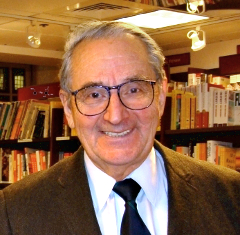
\includegraphics[width=\linewidth]{images/book3/corey.jpg}
\end{minipage}\hfill
\begin{minipage}[t]{0.76\linewidth}
\vspace{0pt}
Os químicos sempre raciocinaram às avessas a partir de seus alvos, mas Elias James Corey, a partir dos
anos 1960, transformou o hábito em regras explícitas: a \omterm{def:b2:retrosynthesis:disconnection}{desconexão}, o \omterm{def:b2:retrosynthesis:disconnection}{sínton}, a seta retrossintética, e
até programas de computador que as aplicavam. Ele recebeu o Prêmio Nobel de Química de 1990 pela teoria
e metodologia da síntese orgânica. (Fotografia: por Trvthchem, CC0, Wikimedia Commons.)
\end{minipage}
\end{history}

\begin{safety}{\ghs[5mm]{GHS02}\,\ghs[5mm]{GHS03}\,\ghs[5mm]{GHS05}\,\ghs[5mm]{GHS06}\,\ghs[5mm]{GHS07}\,\ghs[5mm]{GHS08}}
O cloreto de oxalila é corrosivo, tóxico e reage com a água, liberando cloreto de hidrogênio; a
oxidação de Swern libera monóxido de carbono e sulfeto de dimetila malcheiroso, de modo que é conduzida
na capela. O periodinano de Dess--Martin é um oxidante e não deve ser aquecido. Os reagentes de
cromo(VI) são hoje evitados quando existe uma alternativa.
% ledger: ghs:oxalyl-chloride, ghs:DMSO, ghs:DMP
\end{safety}

\section{Exercícios}

\begin{exercise}[$\star$]\label{exo:b2:retrosynthesis:1}
Desconecte cada álcool em um composto carbonílico e um reagente de Grignard (dê todas as possibilidades):
2-fenilpropan-2-ol, pentan-3-ol, 1-ciclo-hexiletanol, 2-metilbutan-2-ol, 1-feniletanol.
\end{exercise}

\begin{exercise}[$\star$]\label{exo:b2:retrosynthesis:2}
Para a \omterm{def:b2:retrosynthesis:disconnection}{desconexão} do 1-feniletanol na ligação \ce{C-C}, dê os dois \omterm{def:b2:retrosynthesis:disconnection}{síntons}, diga qual é o doador, e dê
um \omterm{def:b2:retrosynthesis:disconnection}{equivalente sintético} para cada um.
\end{exercise}

\begin{exercise}[$\star$]\label{exo:b2:retrosynthesis:3}
Uma via de cinco etapas tem rendimentos por etapa de 90, 85, 80, 95 e 70~\%. Calcule seu rendimento global.
\end{exercise}

\begin{exercise}[$\star$]\label{exo:b2:retrosynthesis:4}
O 4-oxopentanoato de etila deve ser transformado em 5-hidroxipentan-2-ona. Planeje a via com um grupo
protetor, e diga por que ele é necessário.
\end{exercise}

\begin{exercise}[$\star\star$]\label{exo:b2:retrosynthesis:5}
Proponha uma retrossíntese do butano-1,3-diol a partir de compostos com no máximo dois carbonos, com
uma IGF e uma \omterm{def:b2:retrosynthesis:disconnection}{desconexão} a dois grupos.
\end{exercise}

\begin{exercise}[$\star\star$]\label{exo:b2:retrosynthesis:6}
Desconecte a 1-(ciclo-hex-3-en-1-il)etan-1-ona por uma \omterm{def:b2:frontier-orbitals:diels-alder}{reação de Diels--Alder}.
\end{exercise}

\begin{exercise}[$\star\star$]\label{exo:b2:retrosynthesis:7}
Desconecte a 4,4-dimetilciclo-hex-2-en-1-ona por uma \omterm{def:b2:conjugate-additions:robinson}{anelação de Robinson}.
\end{exercise}

\begin{exercise}[$\star\star$]\label{exo:b2:retrosynthesis:8}
A 1-fenilbutan-1-ona pode ser preparada em uma etapa por uma \omterm{def:b2:aromatic-substitution:friedel-crafts}{acilação de Friedel--Crafts}, ou em duas a
partir do benzaldeído. Escreva as duas vias e compare-as.
\end{exercise}

\begin{exercise}[$\star\star$]\label{exo:b2:retrosynthesis:9}
Deseja-se o hexanal a partir do hexan-1-ol. Que reagentes o fornecem, e qual deles daria em vez disso o
ácido hexanoico? Explique.
\end{exercise}

\begin{exercise}[$\star\star\star$]\label{exo:b2:retrosynthesis:10}
No 4-aminobutan-1-ol, a amina deve reagir primeiro com um \omterm{def:b2:acyl-substitution:derivative}{cloreto de acila} em uma etapa, e o álcool
mais tarde com outro. Proponha um par ortogonal de grupos protetores e a sequência.
\end{exercise}

\begin{exercise}[$\star\star\star$]\label{exo:b2:retrosynthesis:11}
Proponha uma síntese da hexano-2,5-diona, um composto 1,4-dicarbonílico, a partir do 3-oxobutanoato de etila.
\end{exercise}

\begin{exercise}[$\star\star\star$]\label{exo:b2:retrosynthesis:12}
A 6-metil-hept-5-en-2-ona, \ce{(CH3)2C=CHCH2CH2COCH3}, é um intermediário de perfumaria. Proponha um
plano completo a partir do 3-oxobutanoato de etila e de um haleto: retrossíntese, via direta, e a etapa
que remove o éster.
\end{exercise}

\section{Problema: A cetona de framboesa}

\begin{problem}[{Problema de fim de semana --- a retrossíntese de um composto aromatizante, o fenol e
a questão de protegê-lo, uma alternativa com paládio, e o julgamento das vias}]
\label{pb:b2:retrosynthesis:1}
A cetona de framboesa, 4-(4-hidroxifenil)butan-2-ona, é encontrada nas framboesas e em outras frutas e
é usada como aromatizante e em perfumaria. Dados do exercício: rendimentos por etapa da via \omterm{def:b2:enolates-aldol:aldol}{aldólica},
85~\% (condensação) e 92~\% (hidrogenação). Massas molares (\unit{g/mol}): C 12.011, H 1.008, O 15.999,
N 14.007, I 126.90. O $\mathrm pK_a$ do fenol é 9.99.
% ledger: use:raspberry-ketone, aw:C, aw:H, aw:O, aw:N, aw:I, pka:phenol, ghs:raspberry-ketone, ghs:4-iodophenol, ghs:MVK

\medskip
\noindent\textbf{Parte I --- Retrossíntese.}
\begin{enumerate}
  \item Desenhe o alvo e dê seus grupos funcionais.
  \item Que IGF transforma a unidade \ce{ArCH2CH2CO} em um padrão com uma \omterm{def:b2:retrosynthesis:disconnection}{desconexão} conhecida?
  \item Escreva a cetona insaturada obtida, com sua geometria.
  \item Que padrão a dois grupos ela contém, e que reação o cria?
  \item Dê os dois materiais de partida.
  \item Por que essa \omterm{def:b2:enolates-aldol:aldol}{aldólica} cruzada dá um produto principal?
  \item Escreva a via direta em duas etapas, com as condições.
\end{enumerate}

\medskip
\noindent\textbf{Parte II --- O fenol.}
\begin{enumerate}[resume]
  \item Em hidróxido de sódio aquoso, em que forma se encontra o 4-hidroxibenzaldeído? Use o
        $\mathrm pK_a$.
  \item Como essa forma muda a eletrofilicidade do aldeído?
  \item Se o fenol fosse protegido, que grupo a segunda etapa removeria de graça? Explique.
  \item Conte as etapas da via com essa proteção.
  \item O anel benzênico corre risco na hidrogenação?
  \item Proteger ou não? Conclua.
\end{enumerate}

\medskip
\noindent\textbf{Parte III --- Uma alternativa com paládio.}
\begin{enumerate}[resume]
  \item Desconecte a cetona insaturada na ligação entre o anel e a cadeia: que parceiros de
        Heck?
  \item Escreva a reação de Heck com trietilamina como base.
  \item Em que carbono da but-3-en-2-ona o grupo arila termina, e por quê?
  \item Dê as etapas do \omterm{def:b2:catalytic-cycles:cycle}{ciclo catalítico}.
  \item Calcule a economia atômica da etapa de Heck, contando a trietilamina.
  \item Calcule a economia atômica da \omterm{def:b2:enolates-aldol:aldol}{condensação aldólica}.
\end{enumerate}

\medskip
\noindent\textbf{Parte IV --- Julgar as vias.}
\begin{enumerate}[resume]
  \item Qual é a economia atômica da hidrogenação?
  \item Calcule a economia atômica global da via \omterm{def:b2:enolates-aldol:aldol}{aldólica}.
  \item Que ligação dupla a hidrogenação reduz, e por que a cetona sobrevive?
  \item Compare os reagentes das duas vias quanto ao custo e ao perigo.
  \item Que via você escolheria?
  \item O que uma terceira etapa a 90~\% faria ao rendimento global?
  \item Dê o rendimento global da via \omterm{def:b2:enolates-aldol:aldol}{aldólica} em duas etapas.
\end{enumerate}
\end{problem}
